\subsubsection{The hollow sphere benchmark}

\label{sec:cookbooks-hollow-sphere}

This benchmark is based on Thieulot \cite{THIE17} in which an analytical solution to the
isoviscous incompressible Stokes equations is derived in a spherical shell geometry.
The velocity and pressure fields are as follows:

\begin{eqnarray}
v_r(r,\theta)      &=& g(r) \cos \theta, \\
v_\theta(r,\theta) &=& f(r) \sin \theta, \\
v_\phi(r,\theta)   &=& f(r) \sin \theta, \\
p(r,\theta)        &=& h(r) \cos \theta ,
\end{eqnarray}
where
\begin{eqnarray}
f(r) &=& \frac{\alpha}{r^2} + \beta r, \\
g(r) &=& -\frac{2}{r^2} \left(  \alpha \ln r + \frac{\beta}{3}  r^3  + \gamma \right),   \\
h(r) &=& \frac{2\mu_0}{r} g(r),
\end{eqnarray}
with
\begin{eqnarray}
\alpha&=&-\gamma \frac{R_2^3-R_1^3}{R_2^3 \ln R_1 - R_1^3 \ln R_2}, \\
\beta &=& -3\gamma \frac{\ln R_2 - \ln R_1  }{R_1^3 \ln R_2 - R_2^3 \ln R_1}.
\end{eqnarray}
These two parameters are chosen so that $v_r(R_1)=v_r(R_2)=0$, i.e.
the velocity is tangential to both inner and outer surfaces.
The gravity vector is radial and of unit length, while the density is given by:
\begin{equation}
\rho(r,\theta)=  \left(   \frac{\alpha}{r^4}  (8 \ln r -6) +  \frac{8\beta}{3r}  +8 \frac{\gamma}{r^4}  \right) \cos\theta.
\end{equation}
We set $R_1=0.5$, $R_2=1$ and $\gamma=-1$. The pressure is zero on both surfaces so that
the surface pressure normalization is used. The boundary conditions that are used are simply
the analytical velocity prescribed on both boundaries.
The velocity and pressure fields are shown in Fig.~\ref{fig:hollow-sphere-vp}.

Fig.~\ref{fig:hollow-sphere-errors} shows the
velocity and pressure errors in the $L_2$-norm as a function of the mesh size $h$ (taken in this case
as the radial extent of the elements). As expected we recover a third-order convergence rate for the velocity
and a second-order convergence rate for the pressure.

\begin{figure}
\centering
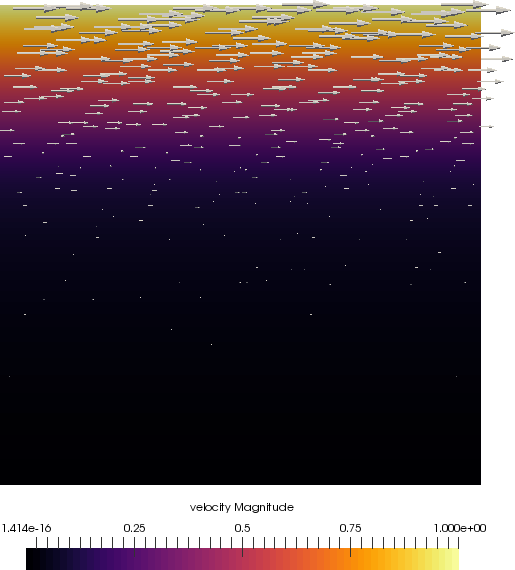
\includegraphics[width=.3\textwidth]{cookbooks/benchmarks/hollow_sphere/doc/vel.png}
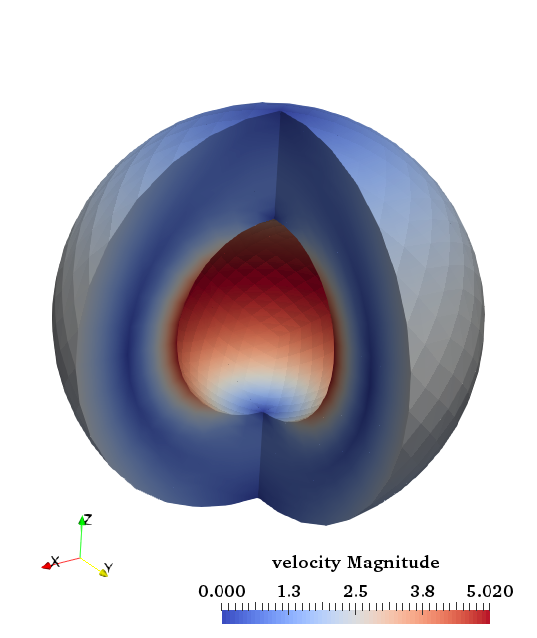
\includegraphics[width=.3\textwidth]{cookbooks/benchmarks/hollow_sphere/doc/vel2.png}
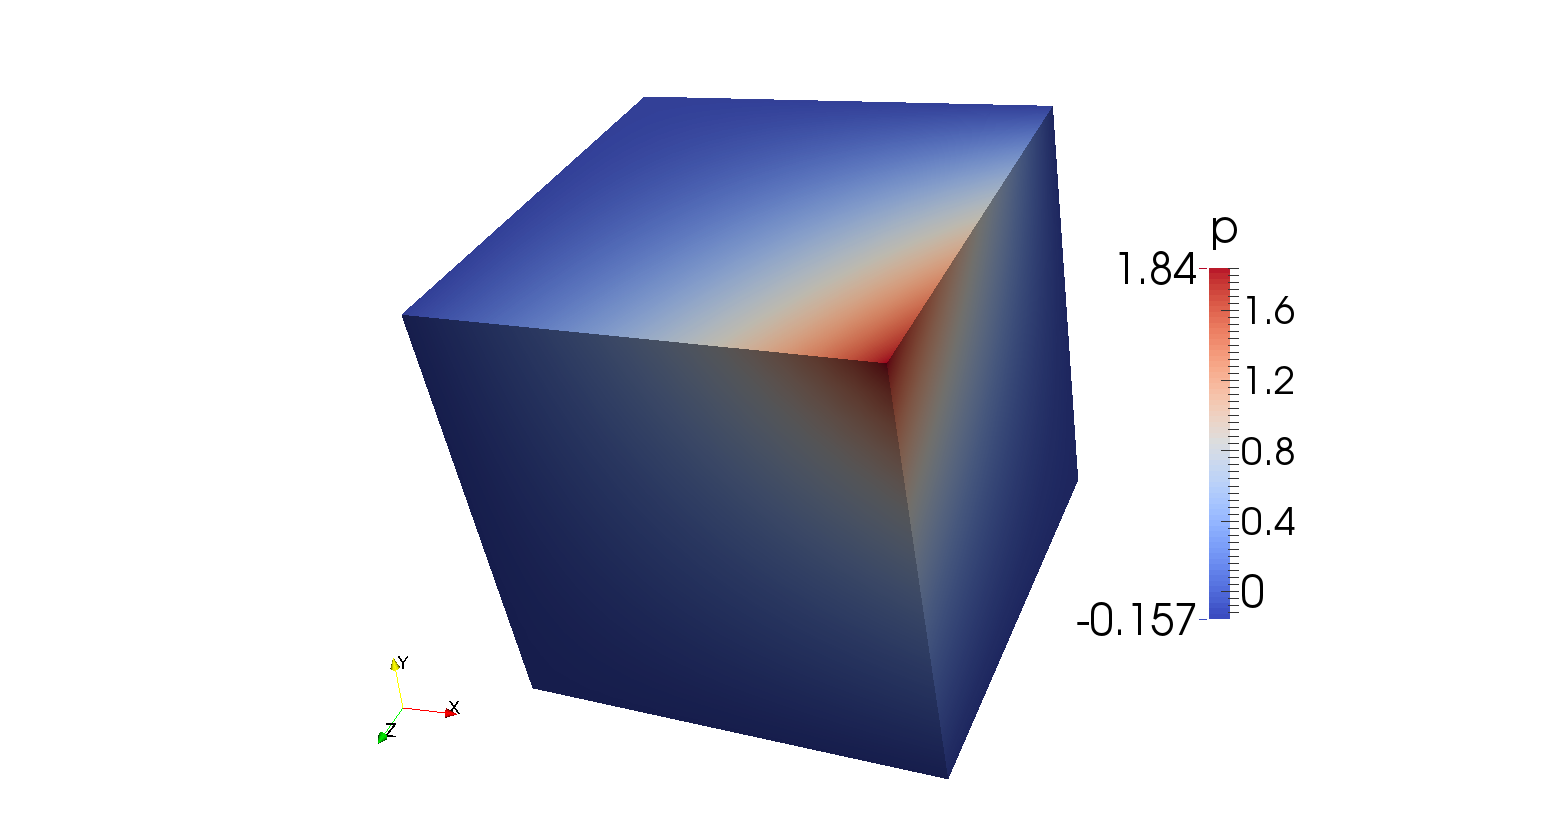
\includegraphics[width=.3\textwidth]{cookbooks/benchmarks/hollow_sphere/doc/pressure.png}
\caption{\it Velocity and pressure fields for the hollow sphere benchmark.}
\label{fig:hollow-sphere-vp}
\end{figure}

\begin{figure}
\centering
\includesvg[width=.7\textwidth]{cookbooks/benchmarks/hollow_sphere/doc/errors_hollowsphere.svg}
\caption{\it Velocity and pressure errors in the $L_2$-norm as a function of the mesh size.}
\label{fig:hollow-sphere-errors}
\end{figure}
